        \subsection{Theorie over het Les geven aan Neurodivergenten-Leerlingen}
            Neurodivergeten leerlingen hebben andere strugels dan hun neurotypisch leerlingen, dat heb ik inmiddels al vijf keer gezegd. Maar wat zijn deze struggles, en wat zijn strategien die we toe kunnen passen om deze struggles te verminderen? De ene manier om deze vraag te beandwoorden is door het eerst op te breken in de verschillende soorten van neurodivergentie\cite{neurodivergent-types}. 

            % ------------------------------------------------------------------
            \subsubsection{ADHD}

                \paragraph{ADHD: Struggles}\\
                    Hoewel ADHD veel symptomen en struggels heeft gaan we het hier vandaag alleen hebben over de struggles die van toepassing zijn op de les omgeving:
                    \begin{itemize}
                    
                        \item \textbf{Wanorde en problemen met prioriteren}: 
                            Mensen met ADHD kunnen eigenlijk alleen taken doen die hun stimuleren. Als de taak dat niet is, is het bijna onmogelijk om je te concentrenen op deze taak. Een taak is snel stimulerend als het urgent is. Dit is omdat de taak leid tot het loslaten van adrealine. Doordat niet stimulerenende taken eigenlijk pas mogelijk worden zodra ze urgent worden zijn belangrijken taken vaak niet aan de orde, ze zijn namelijke nog niet urgent. Pas wanneer ze urgent worden, worden ze stimulerened genoeg om te kunnen doen. Hierdoor is er vaak een mismatch met wat belangrijk is en met wat urgent is, vandaar de problemen met prioriteren.\emph{\hyperlink{https://www.youtube.com/watch?v=5xbD9t8cM4M}{Deze video}}\cite{ADHD-video-prioriteiten} legt heel goed uit waarom dit zo moeilijk is.
                        
                        \item \textbf{Slechte tijdmanagementvaardigheden}: 
                            omdat mensen met ADHD vaak zitten te wachten — zo voelen niet-stimulerende-taken vaak namelijk -, of juist zitten te hyperfocusen omdat iets wel stimulerened is en de tijd voorbij vliegt. Verschilt de perceptie in hoe snel tijd gaat veel op een dag. Hierdoor is het lastig voor mensen met ADHD om de tijd bij te houden. Daardoor hebben ze vaak een slechte time management. 
                        
                        \item \textbf{Problemen met het concentreren op een taak}: 
                            als een taak niet stimulerend is is het bijna onmogelijk om je te kunnen concentreren op deze taak. Dit is omdat je brein meer stimulatie en dopamine nodig heeft om te kunnen functioneren. Hierdoor raak je snel afgeleid sinds je automatisch met taken die je wel stimuleren. Als een soort van junkie trekt je brein naar dingen die wel de stimulatie geven die het nodig heeft.
                        
                        \item \textbf{Moeite met multitasking}: 
                            ieder brein heeft een bepaalde hoeveelheid werk geheugen. Dit is de hoeveelheid dingen die je in je hoofd kan houden. Bij mensen met ADHD is deze hoeveelheid lager. Dat betekend dat mensen met ADHD minder dingen te gelijker tijd kunnen herinneren en daarmee word multitasken moeilijk dan wel ommogelijk. \emph{\hyperlink{https://www.youtube.com/watch?v=HszXKZO_H18&ab_channel=HowtoADHD}{Deze video}}\cite{ADHD-video-working-memory} legt het heel goed uit
                        
                        \item \textbf{Overmatige activiteit of rusteloosheid}: 
                            omdat mensen met ADHD graag bezig zijn en gestimuleerd worden is het lastig voor ons om soms stil te zitten en rust te nemen.
                        
                        \item \textbf{Slechte planning}: 
                            dit is lastig voor ieder tiener brein, dat weet iedereen. Het probleem ligt alleen omdat mensen met ADHD niet snel kijken naar de toekomst (dit is namelijk niet urgent/stimulerend genoeg) hebben ze nooit de skill ontwikkeld om in de toekomst te kijken, en daarvoor te plannen. 
                        
                        \item \textbf{Problemen met het afronden van taken}: 
                            als taken niet stimuleren genoeg zijn kan het zijn dat het dopamine potje opraakt en het brein ergens anders heen moet om dopamine te halen. Hierdoor kunnen mensen met ADHD soms moeilijk taken afroden.
                        
                        \item \textbf{Emotionele regulatie}: 
                            de skill om emoties te behandelen en terug te komen naar de default state is lastiger voor mensen met ADHD. Dit uit zich in:
                            \begin{itemize}
                                \item intensere emoties
                                \item blijven hangen in die intense emoties
                                \item moeite met het omgaan met stress
                                \item snel voelen van emoties (die vervolgens heel intense zijn). 
                                \item Rejection Sensitivity, meer hierover kun je \hyperlink{https://www.youtube.com/watch?v=ZQ44ynEjsHQ&ab_channel=KatiMorton}{\emph{hier}}\cite{ADHD-video-rejection-sensitivity} zien, of \hyperlink{https://my.clevelandclinic.org/health/diseases/24099-rejection-sensitive-dysphoria-rsd}{\emph{hier}} lezen\cite{ADHD-rejection-sensitivity}.
                            \end{itemize}
                \end{itemize}
                
                % — — — — — — — — — — — — — — — — — — — — — — — — — — — — — — — 
                \bigskip
                \noindent\paragraph{ADHD: Sterktes}\\
                    Gelukkig heeft ADHD ook een hoop sterkte punten. We gaan wel weer alleen in op de sterkte punten die relevant zouden kunnen zijn voor onze hypotetische les die we dadelijk gaan ontwerpen.
                    \begin{itemize}
                    
                        \item \textbf{Hyperfocus}:
                            als je je leerlingen engaged en gestimuleerd kan krijgen is het mogelijk ze in hyper focus te krijgen. Als een leeraar leert hoe hij dit in diens leerlingen kan oproepen kan dat een goed sterkte punt zijn en leiden tot goede resultaten.

                        \item \textbf{ADHD Hardnekkigheid}:
                            mensen met ADHD zijn vaak veel vol houdender dan hun neurotypische counterparts. Dit komt omdat ze vaak meer moeite moeten doen om de zelfde taak te voltooien. Hierdoor geven mensen met ADHD vaak minder snel op, ze zijn namelijk gewend dat het niet meteen lukt.\cite{ADHD-resilience}

                        \item \textbf{Sociaal}: 
                            mensen met ADHD zijn over het algemeen veel socialer dan Neurotypische mensen. 

                        \item \textbf{Creatief}: 
                            dit is waarschijnlijk het meest bekende voordeel. Mensen met ADHD zijn vaak veel creatiever dan mensen zonder.\cite{ADHD-creativity}

                        \item \textbf{Visuele denkers}: 
                        mensen met ADHD denken veel visueler
                        
                    \end{itemize}
                    
                % — — — — — — — — — — — — — — — — — — — — — — — — — — — — — — — 
                \bigskip
                \noindent\paragraph{ADHD: Leer tips}\\
                enkele tips die ik gevonden heb bij het les geven van mensen met ADHD zijn:
                \begin{itemize}
                
                    \item \textbf{Duidelijke Instructies Geven}: 
                        \textit{Bied duidelijke, stapsgewijze instructies en herhaal of herschrijf ze indien nodig}. Visuele hulpmiddelen en schriftelijke instructies kunnen nuttig zijn\cite{ADHD-visual}. ADHD'ers leren vaak met hun rechter brein. Hierdoor zijn ze veel visueler en leren ze beter als ze het zien of doen over het horen. Een ander voorbeeld is omdat mensen met ADHD een kleinere hoeveelheid werk geheugen hebben kan het zijn dat ze het nodig hebben om dingen opnieuw te kunnen lezen. Ik zal een voorbeeld geven waarin dit terug komt. 

                        \smallskip
                    
                        Laten we zeggen dat een persoon zonder ADHD 4 dingen tegelijkertijd kan onthouden, en iemand met ADHD maar 3. Als je dan een vraag zou stellen aan beide leerlingen neem je een plek in beslag in dit werk geheugen. De niet-ADHD'er heeft er nog 3 over en de ADHD'er nog maar 2. Geef ze dan 3 mogelijke andwoorden op deze vraag en je hebt een probleem. Het hoofd van de normale leerling zit vol (1 vraag plus 3 andwoorden is 4, het maximale wat hij kan onthouden). Maar de ADHD leerling? Die is inmiddels de vraag vergeten. Je gaf 'm namelijk een vierde ding om te onthouden terwijl die er maar physiek 3 kan onthouden. Dit is wanneer de mogelijkheid om terug te kunnen lezen belangrijk kan zijn voor ADHD leerlingen.\cite{ADHD-video-working-memory}

                    \item \textbf{Visuele Ondersteuning Gebruiken}: 
                        \textit{Geef visuele schema's, grafieken en diagrammen}. Dit brengt ons terug op punt 1. Omdat ze visuele leerlingen zijn is het vaak handing om: 
                        \begin{itemize}
                            \item \textbf{Belangrijke dingen te kleuren en te markeren}. 
                                Dit help visueel de belangrijkste dingen uit elkaar te houden.
                            \item \textbf{oudere kinderen te leren hoe ze informatie kunnen visualieseren in diagramen}. 
                                Neem een voorbeeld aan een mind map. Deze heb ik persoonlijk altijd een investeering gevonden. Handig, maar wel tijd consumerend. Jongeren kinderen kun je laten teken wat ze aan het leren zijn. Op deze manier moeten ze de tijd en moeite nemen om het visueel voor te stellen. 
                        \end{itemize}
                        
                        Deze goede voorbeelden kwamen van \emph{\hyperlink{https://www.additudemag.com/visual-learner-homework-help/}{additudemag.com}}. Je kan precieze link vinden in the references onder nummer \cite{ADHD-visual}.
                    
                    \item \textbf{Taken Opsplitsen in Kleinere Stappen}: 
                        \textit{Verdeel complexe taken in kleinere, beheersbare stappen om overweldiging te voorkomen}. Omdat het werkgeheugen minder is, is het belangrijk dat je helpt met het eerst opslitsen van het probleem. Hierdoor raakt het hoofd van mensen met ADHD minder vol, en voorkom je een overload. Dit herkent iedereen wel. Dit is wanneer het je allemaal even te veel word en je brein het niet meer doet. Er zijn namelijk te veel dingen die je moet doen en je weet niet meer waar je mee moet beginnen. Deze drempel ligt bij mensen met ADHD lager. Daarom is het belangrijk dat je ze helpt met hoe ze dit zelf kunnen doen.
    
                        \smallskip
    
                        Een andere goede suggestie die gemaakt werd door \emph{\hyperlink{https://www.additudemag.com/visual-learner-homework-help/}{additudemag.com}} (zie reference \cite{ADHD-visual}) was om een \textit{Plan-of-Attack} te maken. Gezien het soms moeilijk kan zijn voor ons alle dingen op een rijtje te kunnen zetten. \textit{bullet list} zijn ook een super goede om toe te passen. Op deze manier kan je snel terug kijken of je niet iets vergeten bent.

                    \item \textbf{Een Zintuigvriendelijke Omgeving Creëren}: 
                        \textit{Creëer een comfortabele klasomgeving door rekening te houden met zintuiglijke gevoeligheden}. Bied zintuiglijke hulpmiddelen of ruimtes voor zelfregulering. Mensen met ADHD kunnen sneller over, of onder prikkeld worden. Het is belangrijk om de juiste hoeveelheid prikkels te bieden aan het brein en dit regelmatig te houden. Hoe ik dit bijvoorbeeld doe is het zelfde nummer op repeat te houden. Omdat dit je brein stimuleerd maar er toch ritme in zit houd je toch een soort van rust in je hoofd. Omdat het het zelfde nummer is word het heel voorspelbaar, en voor mij heel prettig.

                    % \item \textbf{Zelfvertegenwoordiging Aanmoedigen}: 
                    %     \textit{Leer studenten hun behoeften te identificeren en te pleiten voor passende aanpassingen of strategieën}. Zij zijn althans de studenten met ADHD, laat hun feedback geven of de stimulatie te veel, of te weinig is, de taak te groot of te klein is, of er te veel, of niet genoeg chaos is.

                    \item \textbf{Regelmatig Feedback Geven}: 
                        \textit{Geef specifieke, constructieve feedback en lof om positief gedrag en prestaties te versterken}. Mensen met ADHD hebben behoefte aan snelle feedback. Het prettigste is om meteen feedback te krijgen of iets goed of fout was. Hierdoor krijg je meteen de dopamine die ons brein vereist om verder te gaan. Als we te lang moeten wachten kan dit leiden tot een concentratie, of motivatie problemen. Het probleem is namelijk niet stimulerend genoeg.
                    
                \end{itemize}

            
    
            % ------------------------------------------------------------------
            \subsubsection{Autisme}
               Autisme en ADHD gaan bijna hand in hand. 50\% tot 70\% van de mensen met autisme heeft ook ADHD\cite{ADHD-en-autisme-overlap}. Dit leid er dan ook toe dat beide zelfde zwaktes en sterke punten hebben.\\
    
                \noindent\paragraph{Autisme: Struggles}\\
                    We gaan wederom de zwakke kanten die niet relevant zijn voor het onderwijs weg laten voor de lengte. Dit mag dan wel een passie essay zijn maar we gaan al richting de 10 pagina's en ik ben nog lang niet klaar.
                    \begin{itemize}
                        \item \textbf{social anxity}: 
                            mensen met autisme hebben vaak moeite, vinden het eng om met mensen contact te maken. Persoonlijk denk ik niet dat dit een ding is dat autisme veroorzaakt maar omdat iemand met autisme vaak niet begrepen word door leeftijds genoten, en misschien zelf leeftijds genoten niet begrijpt word er een soort weerstand opgebouwd met interacties met leeftijds genoten. Want als het eerst niet goed ging, waarom zou het dan nu wel goed gaan?

                            \smallskip

                            Ik bedoel hier niet mee dat het even makkelijk is voor iemand met autisme als iemand zonder om een connectie te leggen. Want gezien je letterlijk op een andere manier je brein hebt opgebouwd is dit zeker niet het geval. Maar ik hoop door het onderwijs beter te maken voor mensen met autisme dat dit in de toekomst te minimaliseren. Het zal namelijk niet 100\% gelijk worden. Maar dat hoeft ook kan ook niet, en dat hoeft ook niet. Zolang als het maar beter, en makkelijker word.
                        
                        \item \textbf{Emotionele regulatie}: 
                            vergelijkbaar met ADHD hebben mensen met autisme last van het reguleren van hun emoties. Dit maakt hun emoties, intenser en langer duurend dan hun neurotypische counterparts. Dit uit zich dan ook in verschillende kenmerken:

                            \begin{itemize}
                                \item druk maken om "niks"
                                \item obsessive compulsive behaviour (OCD)
                                \item meltdowns
                                \item phobias
                            \end{itemize}

                            om dit te voorkomen leerd het brein dingen aan om de emoties te voorkomen in plaats van te leren dealen met deze emoties. Voorbeelden hiervan zijn:

                            \begin{itemize}
                                \item hyper-vigilance, of “shell shocked” lijken
                                \item vermijdend gedrag
                                \item routines en weerstand aan veranderingen
                                \item controlerend gedrag
                                \item of in opstand komen tegen gezag
                            \end{itemize}

                        \item \textbf{shut downs}\cite{autisme-shutdowns}: Dit gebeurd wanneer iemand met autisme overloaded raakt.
                        
                    \end{itemize}
                    
                % — — — — — — — — — — — — — — — — — — — — — — — — — — — — — — — 
                \bigskip
                \noindent\paragraph{Autisme: Sterktes}
                    \begin{itemize}
                        
                        \item \textbf{Focused leren}\cite{autisme-upsides}: 
                            vergelijkbaar met ADHD's hyperfocus kan iemand met autisme de wereld kompleet vergeten en opgaan in waar ze mee bezig zijn.
                            
                        \item \textbf{creativiteit en unique perspecitiven}\cite{autisme-upsides}:
                            Kinderen met autisme hebben vaak een unique blik op iets. Gezien hun brein anders is opgebouwd, en anders informatie verwerkt krijg je natuurlijk ook een andere output!

                        \item \textbf{empathie}\cite{autisme-upsides}: 
                            in tegen stelling tot wat andere denken hebben mensen met autisme meer empathie dan hun neurotypische tegenliggers. Deze mythe komt doordat het moeilijk is om neurotypische mensen om de informatie uit de persoon met autisme te halen.

                        \item \textbf{beter geheugen}\cite{autisme-upsides}: 
                            mensen met autisme hebben vaak een heel goed geheugen. Zeker voor details of patronen. Dit is een van de sterkste kanten van iemand met autisme.

                        \item \textbf{oog voor detail}\cite{autisme-upsides}: 
                            niet alleen kunnen mensen met autisme goed details onthouden, het spotten van details gaat ze heel makkelijk af. Ze zien deze veel beter dan hun neurotypische tegenliggers.
                            
                        \item \textbf{Harnekkigheid}\cite{autisme-upsides}:
                            net zoals ADHD'ers zijn mensen met ADHD hardnekkig en geven ze niet zomaar op. Zekere niet als ze een passie hebben voor iets en ze in hyperfocus gaan.
                            
                    \end{itemize}                    
                    
                % — — — — — — — — — — — — — — — — — — — — — — — — — — — — — — — 
                \bigskip
                \noindent\paragraph{Autisme: Les tips}
                    \begin{itemize}
                        \item \textbf{Structuur en Routine}\cite{autisme-teaching-them}:
                            Het is voor mensen mte autisme heel belangrijk om structuur en routine te hebben. Dit houd ze gefocusd op de taak en zorgt dat ze zich geen zorgen hoeven te maken over kleinen dingen. Een voorbeeld is om na ieder vak kinderen hun spullen op te laten ruimen. Dit geeft dan mentaal het einde van het onderwerp aan. Dit houd het klaslokaal schoon, en structuur in ons hoofd.
                            
                        \item \textbf{Vermijd stimulerende factoren}\cite{autisme-teaching-them}:
                            Om te voorkoment dat mensen met autisme over prikkeld raken is het belangrijk om te zorgen dat de stimulatie tot een minimum getrokken word.
                            
                        \item \textbf{zeg zo min mogelijk en schrijf dingen op}\cite{autisme-teaching-them}:
                            mensen met autisme zijn visuele leerlingen\cite{autisme-visual}. Dus net zoals met ADHD helpt het om:
                                \begin{itemize}
                                    \item duidelijke, stapsgewijze instructies te geven. Herhaal of herschrijf ze indien nodig
                                    \item bied visuele hulpmiddelen zoals highlights/markeren, diagramen 
                                    \item geef schriftelijke instructies in plaats van een heel verhaal te vertellen
                                    \item Laat oudere kinderen te leren hoe ze informatie kunnen visualieseren in diagramen.
                                    \item laat jongeren kinderen kun je laten teken wat ze aan het leren zijn. 
                            \end{itemize}
                            zie de hierboven les tips voor ADHD voor meer informatie.
                        
                        \item \textbf{beprek keuzes}\cite{autisme-teaching-them}:
                            Omdat mensen met autisme focusen op details, en heel analytisch denken kan het zijn dat simple keuzes heel moeilijk kunnen zijn. Als je ze bijvoorbeeld een kleur laat kiezen beperk de opties dan tot 3 verschillende kleuren.
                            
                        \item \textbf{creer een-op-een sociale interacties}\cite{autisme-teaching-them}:
                            Door kinderen met autisme de kans te geven om een op een met 

                    \end{itemize}

% ------------------------------------------------------------------
            \subsubsection{Dyslextia}
            
                \paragraph{Dyslextia: Struggles}\\
                \begin{itemize}
                    \item \textbf{Leesvaardigheden}\cite{dyslextia-struggles-and-superpowers}:
                        Dit is waaschijnlijk de meest bekende problemen die mensen met Dyslextia hebben. 

                    \item \textbf{Schrijfvaardigheden}:
                        Dit is waaschijnlijk het andere meest bekende probleem die mensen met Dyslextia hebben.
                        
                    \item \textbf{Het omkeren van letters en cijfers tijdens het lezen (bijvoorbeeld "zag" lezen als "was")}\cite{dyslextia-struggles-and-superpowers}:
                        Een veel voorkomend probleem is het omkeren van letters zoals 'b' en 'd', of 'p' en 'q'. Gezien dit de zelfde letter is maar dan geroteerd, of gespiegeld.
                        
                    \item \textbf{Notities maken in lessen en lezingen}\cite{dyslextia-struggles-and-superpowers}:
                        Gezien het Lezen en Schrijfven al lastig is, is het voor dyslexten bijna onmogelijk om zowel te lezen, schrijven en luisteren te gelijker tijd.
                    
                    \item \textbf{Sequentiële instructies volgen}\cite{dyslextia-struggles-and-superpowers}:
                        Dit heeft wederom te maken met werk geheugen. Mensen met dyslextie hebben er niet perse minder van zoals met ADHD. Maar het is gebleken dat er verschillende soorten werkgeheugen zijn\cite{dyslextia-different-types-of-memory}. Voornamelijk visueel en auditorisch. (theoretisch zijn er meer vormen. Voor elk zintuig een). Om dingen het beste te onthouden moet men zo veel mogelijk van deze te gelijker tijd gebruiken. Dit geeft je de grootste kans iets te herinneren. Hier is het probleem, mensen met dyslextie hebben een dramatisch slechter auditorisch geheugen. Wat dus betekend dat je daar minder op kan leunen, en daarom alleen maar visueel informatie kan op slaan. Dat betekend dan dus dat je als dyslext minder goed dingen kan onthouden. Je kan namelijk maar gebuik maken van een van de twee smaken.
                        
                    \item \textbf{Woorden, zinnen en namen onthouden}\cite{dyslextia-struggles-and-superpowers}:
                        Mensen onthouden woorden, zinnen, en namen voornamelijk auditorisch. Je onthoud het geheugen van hoe het woord, de zin, of die naam ook al weer klonk. Niet hoe je het ookal weer spelde, of hoe het woord er uit zag. Dit maakt dus dat je als dyslext deze dingen minder goed kan onthouden. Zoals uitgelegd in het punt hierboven.
                        
                    \item \textbf{Geschreven lijsten en telefoonnummers memoriseren}\cite{dyslextia-struggles-and-superpowers}:
                        
                    
                    \item \textbf{Woordrekenproblemen begrijpen}\cite{dyslextia-struggles-and-superpowers}:
                        Het probleem hiermee is omdat dyslexten zoals hierboven auditorisch niet goed dingen kunnen onthouden. Het onthouden van dit verhaal waarin zich een reken probleem voorkomt het moeilijker is om deze informatie er uit te halen. Dat heeft niks te maken met dat ze minder goed kunen rekenen, maar het process om deze informatie uit te vissen is gewoon moeilijker voor ons.
                        
                    \item \textbf{Hun ideeën op georganiseerde wijze uitdrukken}\cite{dyslextia-struggles-and-superpowers}:
                        ik wil mijn punt over werk geheugen niet blijven herhalen, maar ik denk dat ik dat nog een keer moet
                        
                \end{itemize}
                
                % — — — — — — — — — — — — — — — — — — — — — — — — — — — — — — — 
                \bigskip
                \noindent\paragraph{Dyslextia: Sterktes}\\
                \begin{itemize}
                    \item \textbf{Seeing the big picture}\cite{dyslextia-struggles-and-superpowers}:
                        Dyslexten zijn beter in de bigger picture zien dan hun neurotypische teggeliggers.
                        
                    \item \textbf{Het vinden van complexen patronen en verstoring}\cite{dyslextia-struggles-and-superpowers}:
                        Vergelijkbaar met het een van de sterkste voordelen van autisme hebben dislexten een voordeel dat ze veel sneller en veel beter complexen patronen, en verstoring in dat patroon kunnen vinden.
                        
                    \item \textbf{Ruimtelijk inzicht en manipulatie}\cite{dyslextia-struggles-and-superpowers}:
                        Dyslexten zijn net zoals de meeste neurodivergente mensen visueel ingesteld. Ze zijn hier ook een stuk beter in dan neurotypicals. Omdat ze niet 
                        
                    \item \textbf{Visual thinking}\cite{dyslextia-struggles-and-superpowers}:
                        Mensen met dyslextie hebben een veel beter ruimtelijk inzicht en denk vermogen. Is dit waarom de letter op het papier bewegen en draaien? Geen idee.
                        
                    \item {\textbf{Thinking outside the box}\cite{dyslextia-struggles-and-superpowers}:
                        hier volgt een letterlijke vertaling van bron \cite{Creativity-and-Dyslexia} over waarom dyslexten creativer zijn:
                        {"\textit{De meeste mensen met dyslexie hebben de neiging om in beelden te denken in plaats van in woorden, dit komt deels door de activatie van delen van de hersenen" (Jones, 2016) die de meeste volwassenen vaak niet gebruiken. Als gevolg daarvan is wat anderen als innovatief of creatief beschouwen voor een dyslecticus vanzelfsprekend.}"}
                        }
                \end{itemize}

                    
                % — — — — — — — — — — — — — — — — — — — — — — — — — — — — — — — 
                \bigskip
                \noindent\textbf{Dyslextia: Les tips}
                    \begin{itemize}
                        \item{\textbf{Gebruik \hyperlink{https://opendyslexic.org/}{OpenDyslextic}}. 
                            Dit is een lettertype speciaal gemaakt voor mensen met dyslextie. Sterker nog. Ik wou alles in dit lettertype schrijven, dit hele document. Alleen hier heb ik 2 uur op verloren omdat ik maar problemen bleef hebben met \LaTeX. Trust me, I really tried. Dat is ook de rede dat dit document niet zwart op wit is. Ik heb geprobeerd het zo dyslextie vriendelijk te maken. 
                            
                            \bigskip
                            
                            \begin{center}
                                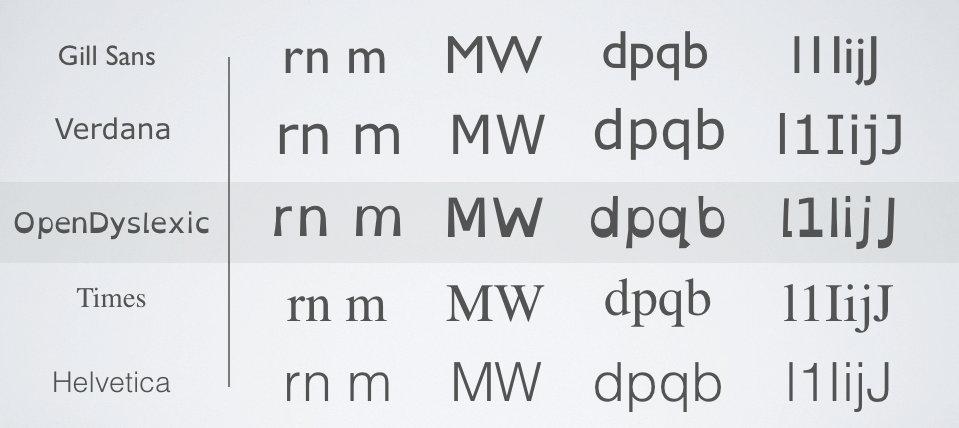
\includegraphics[width=35em]{Eindopdracht-Tygo-van-den-Hurk-1705709/Resources/Images/open-dyslexic-abelardo-gonzalez-font-character-map.png}
                            \end{center}
                            
                            \bigskip
                            
                            \noindent Het is misschien een lelijk lettertype. — Althans dat vond ik in het begin. — Maar heb dit lettertype gebuikt de afgelopen maand het het leest veel fijner naar mijn mening. De eerste paar dagen moest ik echt wennen. Ik moest een soort van op nieuw leren lezen. Maar nu? Nu is het veel veel fijner. Ik gebruik extensies om dit lettertype te forceren. Dit is bijna het enige lettertype dat ik lees.
                            
                            \bigskip
                            
                            \noindent Een probleem dat veel mensen met dyslextie hebben is dat letters draaien en verplaatsen als je ze leest. Zoals je het in de film ziet. — though niet altijd even erg. — Als ik OpenDyslextic gebruik heb ik dit probleem niet meer. Ze blijven gewoon stil staan. Dat niet alleen, Letters lijken ook minder op elkaar.
                            
                            \bigskip
                            
                            \noindent Ik kan niet de enige zijn die ooit heeft opgemerkt dat van deze zes letters: \texttt{p}, \texttt{q}, \texttt{b}, \texttt{d}, \texttt{O}, \texttt{0}; het er maar twee zijn. \texttt{d} \& \texttt{O} zijn allemaal het zelfde. En dat is echt heel irritant. Zeker als je even een mindere dag hebt waar de letters op je papiertje net soep zijn. Kijk OpenDyslexic kan geen wonderen maken, maar kijk naar de afbeelding, ze hebben ze verschillend gemaakt. Dit maakt ze zo veel minder vermoeiend om te lezen.
                            
                            \bigskip
                            
                            \noindent Ze hebben ook funky dingen gedaan met de spacing van de letters etc. Ik kan hier uren over door gaan. Punt is, dit is een upgrade, gebruik het. Als je meer wil weten, of dit lettertype \textbf{gratis} wil downloaden, ga dan naar \underline{\hyperlink{https://opendyslexic.org/}{opendyslexic.org}.
                        }

                        \item{\textbf{Houd het visueel}. 
                            Net zoals bij de tips voor ADHD, en autisme is het belangrijk dat je dingen visueel houd. Zeker gezien lezen vaak een probleem is. Plaatjes, grafieken, en diagramen zijn een god sent.
                        }
                    \end{itemize}

%             % ------------------------------------------------------------------
            \subsubsection{Dyscalculia}
            
                \paragraph{Dyscalculia: Struggles}\\
                    ...
                
                % — — — — — — — — — — — — — — — — — — — — — — — — — — — — — — — 
                \bigskip
                \noindent\paragraph{Dyscalculia: Sterktes}\\
                    ... 
                    
                % — — — — — — — — — — — — — — — — — — — — — — — — — — — — — — — 
                \bigskip
                \noindent\paragraph{Dyscalculia: Les tips}\\
                    ...

%             % ------------------------------------------------------------------
            \subsubsection{Being Queer}
            
                \paragraph{Being Queer: Struggles}\\
                    ...
                
                % — — — — — — — — — — — — — — — — — — — — — — — — — — — — — — — 
                \bigskip
                \noindent\paragraph{Being Queer: Sterktes}\\
                    ... 
                    
                % — — — — — — — — — — — — — — — — — — — — — — — — — — — — — — — 
                \bigskip
                \noindent\paragraph{Being Queer: Les tips}\\
                    ...

        \subsection{Conclusion}
            Er waren een paar dingen die we hiervan kunnen leren. Een paar sterktes waar we op in kunnen spelen, en een paar zwaktes die we zouden moeten kunnen trainen en vermijden.

            \subsubsection{Problemen}
                Ten eerste, de meeste neurodivergente mensen zijn visueel ingeteld. Sterker nog, nadat ik mijn onderzoek heb gedaan blijkt dat 65\% visuele leerlingen zijn.\cite{Visual-Learners-are-the-most-common} Daarom moet ik zorgen dat mijn les voornamelijk visueel is ingesteld. De meeste lessen worden nu gegeven worden, worden gedaan door middel van een iemand die voor de klas staat en een verhaal verteld. Niet super ideaal. Tweede probleem is dat afhankelijk van welk type neurodivergente leerling je hebt, dat je verschillende levels van stimulatie moet hebben. Dus daar moeten we ook iets aan doen
            
            \subsubsection{Oplossingen}
                Okay sinds het meeste visueel zal moeten zullen we moeten zorgen dat dat in orde is. Een white bord zal het niet worden. Afhankelijk van wat we er op willen zetten we extreem veel tijd kwijt zijn. Als deze tijd te lang is raakt die ene ADHD'er in de hoek afgeleid. Mij zien tekenen is niet stimulerend genoeg. Dus we zullen in de voor bereiding sowieso tijd moeten stoppen in het maken van een power-point voor alle concepten die we willen behandelen. Samen met tekeningen. Het voordeel is wel. Zodra we een concept getekend hebben kunnen we deze visuele concepten recyclen. We kunnen ze namelijk ieder jaar over en over gebruiken. 
                
                \bigskip
                
                \noindent Hier is een lijst van dingen die we kunnen gebruiken om ons voorbereide powerpoint whiteboard zo appealling als mogelijk te maken voor onze visuele leerlingen.
                
                \begin{itemize}
                    \setlength\itemsep{0em}
                    \item Schrijf nieuwe vocabulary op, en kleur ze zodat ze opvallen;
                    \item gebruik het whiteboard efficient. We zullen ons digitale whiteboard al van te voren gemaakt hebben
                    \item Gebruik grafieken en diagrammen.
                    \item Voeg symbolen en beweging toe aan flashcards.
                    \item Speel flashcardspellen.
                    \item Experimenteer met realia.
                    \item Gebruik diavoorstellingen en video's.
                    \item Moedig hen aan om vooraan te zitten.
                    \item Gebruik OpenDyslextic.
                \end{itemize}
                
                \bigskip
                
                \noindent Ten tweede hoe krijgen we iedereens stimulatie levens optimaal? Ik bijvoorbeeld heb — de hele dag door — het zelfde nummer op repeat. Omdat het zelfde nummer is zit er structuur in. Bij de 5e keer weet je exact waar wat zit. Maar het is toch stimulerend. Dit werkt alleen niet voor iedereen. De ander heeft absolute stilte nodig.
                
                \bigskip
                
                \noindent Hiervoor hebben we kop telefoons. Iedereen heeft tegenwoordig kop telefoons met noice-cannelation wat betekend dat ze in stilte kunnen werken, als ze dit willen. Daarom ga ik tegen stelling tot wat andere docenten doen, het gebruik van koptelefoons stimuleren. Het houd leerlingen gefocust en afgezonderd van elkaar. Wanneer ze zelf mogen werken, werken ze dus ook alleen.
                
                \bigskip
                
                \noindent Dan hebben we nog het laatste ding. We moeten voorspelbaar zijn. Voorspelbaar en gestrucureerd. Dan weten ze precies wat ze te wachten staat. Daarom moeten we de les planning op het bord schrijven en de leerlingen uit nodigen mij als docent te verbeteren en mij aan de tijd te houden. 
\newpage